\documentclass{article}
\usepackage{amsmath}
\usepackage{amssymb}
\usepackage{graphicx}
\usepackage{geometry}
\usepackage{multicol}
\usepackage{tikz}
\usepackage{pgfplots}

\title{Algorithms \\ CSE 2415}
\author{Md. Hasan}
\date{April 2024}

\begin{document}
\maketitle
\newpage

\section*{Introduction}

Algorithm is a sequence of steps / step-by-step procedure to solve a problem.

\vspace*{20pt}

Properties of Algorithm:

\begin{itemize}
    \item Specific input
    \item Specific output
    \item Definiteness
    \item Finiteness
    \item Effectiveness
\end{itemize}

\section*{Time and Space Complexity}

\textbf{Examples: }

\hrulefill
\begin{multicols}{3}
    \begin{minipage}{\linewidth}
        \section*{}
        % Your content for section 1 goes here
        \begin{verbatim}
Algorithm:

int i, j;
for(i = 0; i < n; i++){
    for(j = 0; j < n; j++)
        printf(" \%d ", i+j);
}
        \end{verbatim}
    \end{minipage}
    
    \begin{minipage}{\linewidth}
        \section*{}
        % Your content for section 2 goes here
        \begin{verbatim}
        space complexity
        cost      repeat      total
         1          1           1
       1+1+1    1+(n+1)+n     2n+2
       1+1+1  (1+(n+1)+n)+n  2n^2+2n
         1         n^2         n^2

        F(n)= 3n^2 + 3n + 1
        TC -> O(n^2)
        \end{verbatim}
    \end{minipage}

    
    \begin{minipage}{\linewidth}
        \section*{}
        % Your content for section 3 goes here
        \begin{verbatim}
            Space complexity
            cost  repeat  total
            i= 4     1     4
            j= 4     1     4
            n= 4     1     4
            

            S(n)= 12
            SC -> O(1)
        \end{verbatim}
    \end{minipage}
\end{multicols}

\newpage
\hrulefill
    \begin{verbatim}
    Algorithm:

    int i, j, n, A[i][j], B[i][j], C[i][j];
    for(i = 0; i < n; i++){
        for(j = 0; j < n; j++)
            C[i][j] = A[i][j] + B[i][j];
    }
    
    space complexity                    Space complexity

    cost      repeat       total         cost  repeat  total
      1          1           1           i=4     1       4
    1+1+1    1+(n+1)+n      2n+2         j=4     1       4
    1+1+1   n+n(n+1)+n^2   2n^2+2n       n=4     1       4
      1         n^2         n^2         A[][]   4*n*n   4n^2
                                        B[][]   4*n*n   4n^2
                                        C[][]   4*n*n   4n^2

    F(n)= 3n^2 + 4n + 3                 S(n)= 12n^2 + 12
     TC -> O(n^2)                        SC -> O(n^2)
\end{verbatim}

\hrulefill
\begin{verbatim}
    Algorithm:

    int i, n;
    for(i = 0; i < n; i++)
        printf(" \%d ", 2*i);
    
    space complexity                    Space complexity

    cost        repeat      total         cost  repeat  total
      1           1           1           i=4     1       4
    1+1+1  1+(n/2)+1+(n/2)   n+2          n=4     1       4
      1          n/2         n/2         

    F(n)= (3n/2) + 3                    S(n)= 8
     TC -> O(n)                          SC -> O(1)
\end{verbatim}

\newpage
\hrulefill
\begin{verbatim}
    Algorithm:

    int p=0, i, n;
    for(i = 1; i <= p; i++)
        p+=1;

    Step analysis:
    i       p
    0      0+1
    1     0+1+2
    2    0+1+2+3
    3   0+1+2+3+4
    .       .
    .       .
    .       .
    k 0+1+2+3+4+...+k = k*(k+1)/2

    assume , p>n where step number is k and p = k*(k+1)/2
            k(k+1)/2 = n
         => k(k+1) = 2n
         => k^2 + k - 2n = 0
         => k^2 = 2n [ removed k as k^2 > k ]
         => k = sqrt(2n)
         => k = sqrt(2) * sqrt(n)

    thus O(sqrt(n))
\end{verbatim}
\hrulefill
\begin{verbatim}
    int i, n;
    for(i =1; i<n; i*=2)
        printf("%d", i);

    Step Analysis:
    
    steps       2*i
     1           1
     2           2
     .           .
     .           .
     .           .
     k           2^k        [actual value is 2^(k-1)]
     
\end{verbatim}
\newpage
\begin{verbatim}
    assume, code stopped at step k where , i  2^k
        2^k > n
      =>2^k = n
      =>log 2^k = log n
      =>k = log n  [log 2 ^ x = x , here base is always 2 causo fo binary ]

      -> O(log n)
\end{verbatim}

\hrulefill
\begin{verbatim}
    int i, n;
    for(i =n; i > 1 ; i/=2)
        printf("%d", i);

    Step Analysis:
    
    steps       i/2
     1           n
     2          n/2
     .           .
     .           .
     .           .
     k          n/2^k  

     n/2^k < 1
   =>2^k < n
   =>2^k = n
   =>log 2^k = log n
   => k = log n
\end{verbatim}
\hrulefill
\begin{verbatim}
    int p=0, i;
    for(i =0; i<n; i*=2)
        p++;              ------> O(log n)
    for(i=p; i>1; i/=2)     '---> p = log n
        printf("%d", i);    '---> O(log log n)
\end{verbatim}
\hrulefill
\newpage
\hrulefill
\begin{verbatim}
                Time Complexity Cheat Sheet
                
    Constant TC   - O(1)         -> for( i=0; i<k; i++ )
                  - O(sqrt(n))   -> for( i=0; p<n; i++ )

    Linear TC     - O(n)         -> for( i=1; i<n; i++ )
                                 -> for( i=0; i<n; i+=2)
                                 -> for( i=n; i>n; i-=5)

    Logarithm TC  - O(log n)     -> for( i=0; i<n; i*=2)
                                 -> for( i=n; i>1; i/=2)
                  - O(log_a n)   -> for( i=1; i<n; i*=a)

    Polynomial TC - O(n^2)       -> for(--) for(--)
                  - O(n^3)       -> for(--) for(--) for(--)

    Exponential TC- O(2^n),O(n^n)-> Any recursive function
 
\end{verbatim}
\hrulefill

\subsection*{Recursion:}

Substitution method:
\begin{verbatim}
    -> It solves all types of recursive problems
    -> It always gives right answers
    -> Takes more time then Master method
\end{verbatim}

Master method:
\begin{verbatim}
    -> It solves Specific types of recursive problems
    -> Format: T(n) = aT(n/b) + f(n) ; where a >= 1 and b > 1

    Different cases:
        1. f(n) < n log_b a ; 
            T(n) = (theta) (n log_b a)

        2. f(n) = n log_b a ; 
            T(n) = (theta) (n log_b a . log n)

        3. f(n) > n log_b a ; 
            T(n) = (theta) (f(n))
\end{verbatim}
\hrulefill
\newpage

\textbf{Examples:}

$EQ^n:$
\[
    T(n) = 
    \begin{cases}
        t(n-1) + n & \text{, } n > 1 \\
        1 & \text{, } n \leq 1
    \end{cases}
\]

$Sol^n:$
We have,
\begin{equation}
    T(n) = t(n-1) + n \quad \text{---(1)}
\end{equation}

Replace \( n \) by \( n-1 \) in equation (1):
\begin{equation}
    T(n-1) = t(n-2) + (n-1) \quad \text{---(2)}
\end{equation}

Putting equation (2) in equation (1) we get,
\begin{equation}
    T(n) = t(n-2) + (n-1) + n \quad \text{---(3)}
\end{equation}

Similarly, replacing \( n \) by \( n-2 \) in equation (1) we get,
\begin{equation}
    T(n-2) = t(n-3) + (n-2) \quad \text{---(4)}
\end{equation}

Putting equation (4) in equation (3) we get,
\begin{equation}
    T(n) = t(n-3) + (n-2) + (n-1) + n \quad \text{---(5)}
\end{equation}

So, the general equation may be,
\begin{equation}
    T(n) = t(1) + 2 + 3 + \ldots + (n-2) + (n-1) + n \quad \text{---(6)}
\end{equation}

Given \( T(1) = 1 \) we get from  equation (6),
\begin{align*}
    T(n) & = t(1) + 2 + 3 + \ldots + (n-2) + (n-1) + n \\
         & = 1 + 2 + 3 + \ldots + (n-2) + (n-1) + n \\
         & = \frac{n(n+1)}{2} \\
         & = \frac{n^2}{2} + \frac{n}{2}
\end{align*}

Here, \( n^2 \) is the time complexity. Thus, the answer is \( O(n^2) \).

\hrulefill

\newpage

$EQ^n:$
\[
    T(n) = 
    \begin{cases}
        t(n/2) + c & \text{, } n > 1 \\
        1 & \text{, } n \leq 1
    \end{cases}
\]

$Sol^n:$
We have,
\begin{equation}
    T(n) = t\left(\frac{n}{2}\right) + c \quad \text{---(1)}
\end{equation}

Replace \( n \) by \( n/2 \) in equation (1):
\begin{equation}
    T\left(\frac{n}{2}\right) = t\left(\frac{n}{4}\right) + c \quad \text{---(2)}
\end{equation}

Putting equation (2) in equation (1) we get,
\begin{equation}
    T(n) = t\left(\frac{n}{4}\right) + c + c \quad \text{---(3)}
\end{equation}

Similarly, replacing \( n \) by \( n/4 \) in equation (1) we get,
\begin{equation}
    T\left(\frac{n}{4}\right) = t\left(\frac{n}{8}\right) + c \quad \text{---(4)}
\end{equation}

Putting equation (4) in equation (3) we get,
\begin{equation}
    T(n) = t\left(\frac{n}{8}\right) + c + c + c \quad \text{---(5)}
\end{equation}

So, the general equation may be,
\begin{equation}
    T(n) = t\left(\frac{n}{2^k}\right) + kc \quad \text{---(6)}
\end{equation}

Assume that in the \( k \)-th step, \( \frac{n}{2^k} = 1 \)
\begin{align*}
    & \Rightarrow \frac{n}{2^k} = 1 \\
    & \Rightarrow n = 2^k \\
    & \Rightarrow \log n = \log 2^k \\
    & \Rightarrow k = \log n
\end{align*}

Using the value of \( k \) in equation (1), we get,
\begin{equation}
    T(n) = t(1) + kc = 1 + (\log n) \cdot c
\end{equation}

Here, \( t(1) \) is the base case complexity. Thus, the answer is \( O(\log n) \).

\hrulefill
\newpage

$EQ^n:$
\[
    T(n) = 
    \begin{cases}
        2t(n/2) + n & \text{, } n > 1 \\
        1 & \text{, } n = 1
    \end{cases}
\]

$Sol^n:$

We have,
\begin{equation}
    T(n) = 2t\left(\frac{n}{2}\right) + n \quad \text{---(1)}
\end{equation}

Replace \( n \) by \( n/2 \) in equation (1):
\begin{equation}
    T\left(\frac{n}{2}\right) = 2t\left(\frac{n}{4}\right) + \frac{n}{2} \quad \text{---(2)}
\end{equation}

Putting equation (2) in equation (1) we get,
\begin{equation}
    T(n) = 2\left(2t\left(\frac{n}{4}\right) + \frac{n}{2}\right) + n
\end{equation}
\begin{equation}
    T(n) = 4t\left(\frac{n}{4}\right) + 2n \quad \text{---(3)}
\end{equation}

Similarly, replacing \( n \) by \( n/4 \) in equation (1) we get,
\begin{equation}
    T\left(\frac{n}{4}\right) = 2t\left(\frac{n}{8}\right) + \frac{n}{4} \quad \text{---(4)}
\end{equation}

Putting equation (4) in equation (3) we get,
\begin{equation}
T(n) = 4(2t\left(\frac{n}{8}\right) + \frac{n}{4}) + 2n
\end{equation}

\begin{equation}
    T(n) = 8t\left(\frac{n}{8}\right) + 3n \quad \text{---(5)}
\end{equation}


So, the general equation may be,
\begin{equation}
    T(n) = 2^k t\left(\frac{n}{2^k}\right) + kn \quad \text{---(6)}
\end{equation}
Given \( T(1) = 1 \),
\begin{align*}
    T(n) & = 2^k T\left(\frac{n}{2^k}\right) + kn \\\text{we get , }
    n & = 2^k && \text{---(a)} \\
    \log n & = \log 2^k \\
    \text{or, } k & = \log n && \text{---(b)} \\
    \text{Since } n = 2^k, \text{ we have } k = \log n \\
    \text{thus, } T(n) & = nT\left(\frac{n}{n}\right) + n \log n && \text{[using equations (a) and (b)]} \\
    T(n) & = n + n\log n\\
\text{thus, we get }    TC &= O(n \log n)
\end{align*}
\hrulefill
\newpage
\textbf{Master Method Examples:}
\vspace*{10pt}

$EQ^n:$
\[
    T(n) = 
    \begin{cases}
        2t\left(\frac{n}{2}\right) + n & \text{, } n > 1 \\
        1 & \text{, } n = 1
    \end{cases}
\]

$Sol^n:$

\[
    a = 2, \quad b = 2, \quad f(n) = n
\]
\[
    n^{\log_b a} = n^{\log_2 2} = n^1 = n
\]

\[
    f(n) = n^{\log_b a}
\]

\begin{align*}
    TC &= \theta (n^{\log_2 2} \cdot \log n) \\
       &= \theta (n \cdot \log n) 
\end{align*}

\hrulefill
\vspace*{10pt}


$EQ^n:$
\[
    T(n) = 
    \begin{cases}
        T\left(\frac{n}{2}\right) + c & \text{, } n > 1 \\
        1 & \text{, } n \leq 1
    \end{cases}
\]

$Sol^n:$

\[
    a = 1, \quad b = 2, \quad f(n) = c
\]
\[
    n^{\log_b a} = n^{\log_2 1} = n^0 = 1
\]

\[
    f(n) = n^{\log_b a}
\]

\begin{align*}
    TC &= \theta (n^{\log_2 1} \cdot \log n) \\
       &= \theta (1 \cdot \log n)\\
       &= \theta (\log n)
\end{align*}

\hrulefill
\vspace*{10pt}

$EQ^n:$
\[
    T(n) = 
    \begin{cases}
        T\left({n-1}\right) + n & \text{, } n > 1 \\
        1 & \text{, } n \leq 1
    \end{cases}
\]

$Sol^n:$
\[
    a = 1, \quad b = 1, \quad f(n) = n
\]  

Since, b is not greater then a, we cant use master method to find the complexity.

\hrulefill
\newpage

\section*{Divide And Conquer Method:}

\textbf{3 step to solve level of problem:}

\begin{verbatim}
    1. Divide:
                Divide the problem into problems into a number of subproblems that are
            similar to the problem.
    2. Conquer:
                Conquer the subproblems by solving them recursively. If the subproblem's
            size is small enough, just solve it in straight forward manner.
    3. Combine:
                Combine the solutions of the subproblems to get the solution of the
            original problem.

Example:
    For MergeSort it works as follows:
        1. Divide the n-element array into two n/2 elements to Sort.
        2. Sort the two subsequences recursively using MergeSort.
        3. Merge the two sorted subsequences.
\end{verbatim}
\hrulefill

\section*{Time Complexity function Comparison:}
\subsection*{Big O cheat sheet}
TC class :
\[1 < \log n < \sqrt{n} < n < n \log n < n^2 < n^3 < \ldots < 2^n < 3^n < \ldots < n^n\]

\begin{center}
    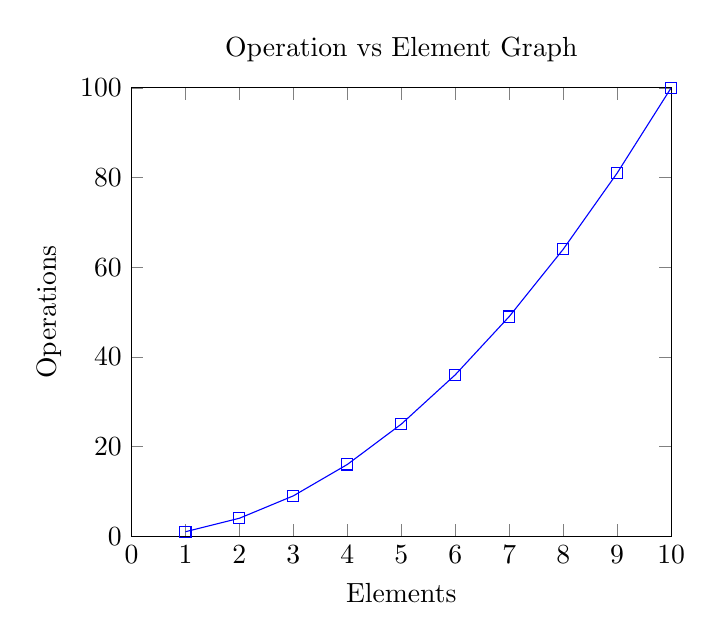
\begin{tikzpicture}
    \begin{axis}[
        title={Operation vs Element Graph},
        xlabel={Elements},
        ylabel={Operations},
        xmin=0, xmax=10,
        ymin=0, ymax=100,
        xtick={0,1,2,3,4,5,6,7,8,9,10},
        ytick={0,20,40,60,80,100},
        legend pos=north west,
        grid style=dashed,
    ]
    
    \addplot[
        color=blue,
        mark=square,
        ]
        coordinates {
        (1,1)(2,4)(3,9)(4,16)(5,25)(6,36)(7,49)(8,64)(9,81)(10,100)
        };
        
    \end{axis}
    \end{tikzpicture}
\end{center}


\end{document}
